\documentclass[letterpaper,final,12pt,reqno]{amsart}

\usepackage[total={6.3in,9.2in},top=1.1in,left=1.1in]{geometry}

\usepackage{bm}
\usepackage{empheq}
\usepackage[dvipsnames]{xcolor}
\usepackage{graphicx}
\usepackage{verbatim,fancyvrb}
\usepackage{tikz}

% hyperref should be the last package we load
\usepackage[pdftex,
colorlinks=true,
plainpages=false, % only if colorlinks=true
linkcolor=blue,   % only if colorlinks=true
citecolor=Red,   % only if colorlinks=true
urlcolor=black     % only if colorlinks=true
]{hyperref}

\renewcommand{\baselinestretch}{1.05}

\newcommand{\eps}{\epsilon}
\newcommand{\RR}{\mathbb{R}}

\newcommand{\grad}{\nabla}
\newcommand{\Div}{\nabla\cdot}
\newcommand{\sgn}{\operatorname{sgn}}
\newcommand{\trace}{\operatorname{tr}}

\newcommand{\bg}{\mathbf{g}}
\newcommand{\bn}{\mathbf{n}}
\newcommand{\bu}{\mathbf{u}}
\newcommand{\bv}{\mathbf{v}}
\newcommand{\bx}{\mathbf{x}}

\newcommand{\bX}{\mathbf{X}}



\begin{document}
%\graphicspath{{figures/}}

\title[Synthetic, time-dependent glacier]{Synthetic, time-dependent glacier \\ for testing surface kinematical inversion}

\author{Ed Bueler}

\maketitle

%\vspace{-8mm}
\begin{center}
{\footnotesize
\emph{version: \today}}
\end{center}

\thispagestyle{empty}

\section{Surface kinematical equations}  We seek to understand how the surface and shape of a glacier evolves, so we consider a flow-line with coordinates $x$ in the horizontal and $z$ in the vertical; there is only one horizontal dimension.  Let $s(t,x)$ be the surface elevation.  For simplicity the bed is flat ($b=0$), so the thickness and surface elevation coincide: $s=h$.  Let $\bn_s(t,x) = \left<-\frac{\partial s}{\partial x},1\right>$ denote the upward normal vector on the ice surface; it is not a unit vector in general.  The scalar slope $\frac{\partial s}{\partial x}$ and the normal vector $\bn_s$ both describe the orientation of the surface.

One may fix time $t$ and visualize $z=s(t,x)$ as a curve in $x,z$ space.  Alternatively, $z=s(t,x)$ can be visualized as a surface in $t,x,z$ space.

At the surface of a glacier the ice has a velocity and the climate adds or removes ice.  Let $\bu(t,x,z)=\left<u,w\right>$ denote the ice velocity, with components $u$ in the horizontal and $w$ in the vertical.  Let $\bu|_s(t,x) = \bu(t,x,s(t,x))$ denote the surface value of the ice velocity.  Let $a(t,x)$ be the climatic (surface) mass balance (CMB), the accumulation-ablation function.  In these terms the traditional \emph{surface kinematical equation} (SKE), also called the ``kinematical boundary condition'' \cite{FowlerNg2021,GreveBlatter2009}, is
\begin{equation}
\frac{\partial s}{\partial t} - \bu|_s \cdot \bn_s - a = 0  \label{ske}
\end{equation}
This equation says that, at times $t$ and locations $x$ where a glacier is present, i.e.~where $s(t,x)>0$, on the surface of the ice there is a balance between the rate of change of the surface elevation, the motion of the ice, and the CMB.  By expanding the dot product it is equivalent to write ``$\frac{\partial s}{\partial t} + u|_s \frac{\partial s}{\partial x} - w|_s - a = 0$'' or ``$\frac{\partial s}{\partial t} = - u|_s \frac{\partial s}{\partial x} + w|_s + a$''; you might see these forms in textbooks.

The new form, the kinematical conservation law (KCL), is integrated in time and space, and it applies everywhere.  It applies not only on the surface of the ice but on the adjacent ice-free land.  The derivation of this new form is given in the early draft titled \emph{A new kinematical conservation law for glaciers}.  To state it here we can consider a one-dimensional domain $\Omega$ which is merely an interval, $\Omega=[x_0,x_1]$, and an interval of time $[t_0,t_1]$.  In these terms the KCL is
\begin{align}
\int_{x_0}^{x_1} h(t_1,x)^2\,dx &= \int_{x_0}^{x_1} h(t_0,x)^2\,dx + 2 \int_{t_0}^{t_1} \int_{x_0}^{x_1} h(t,x)\, \bu|_s(t,x)\cdot \bn_s(t,x) \,dx\,dt \label{kcl} \\
  &\hspace{34mm} + 2 \int_{t_0}^{t_1} \int_{x_0}^{x_1} h(t,x)\, a\left(t,x\right) \,dx\,dt \notag
\end{align}
This form says that the square of the ice thickness is conserved in the sense that at a later time $t_1$ the value is the same as at an earlier time $t_0$, except for the identified total contributions from ice dynamics ($2 \int \int h\, \bu|_s \cdot \bn_s \,dx\,dt$) and CMB ($2 \int \int h\, a \,dx\,dt$).  These contributions are ``weighted'' by the thickness, so thinner ice (small $h$) areas do not contribute much, and ice-free areas do not contribute at all.

The new form is only advantageous if we seek to account for changes in the glacier which occur in locations $x$ where at some times a glacier is present ($h(t,x)>0$) and at other times not ($h(t,x)=0$).  Thus there is no need to track the time-varying region occupied by the glacier, i.e.~the set $R(t) = \{x\,|\,h(t,x)>0\}$.  In particular, we hope to see advantages of the new approach when used in simultaneously inverting for the CMB function $a(t,x)$, the equilibrium line altitude, and the time-dependent glacier outline, from purely kinematical observations of the surface elevation and velocity.


\section{Synthetic glacier formulas}

The significance of the SKE and KCL should become clearer by the construction of an exactly-specified, but synthetic, example.  This example has surface elevation, ice velocity, and CMB which evolve together in a manner so that the SKE and KCL are both exactly satisfied.  (For the SKE we would say more accurately that it is ``exactly satisfied in locations where it applies''.)

The specific synthetic geometry is based on a steady-state ice sheet profile from section 5.3 of \cite{vanderVeen2013}, called the \emph{Bueler profile} and derived in \cite{Bueler2003}.  However, additional time dependence is added through making the center height and length time-varying, so the term $\frac{\partial s}{\partial t}$ is nonzero.  The formulas are based on a few scalar parameters, as in Table \ref{constantstable}.

\begin{table}
\begin{tabular}{clll}
variable  & description & units & value \\
\hline
    & seconds per year &  & 31556926.0 \\
$A$ & ice softness in Glen law & $\text{Pa}^{-3}\,\text{s}^{-1}$ & $10^{-16}/31556926.0$ \\
$g$ & gravity & m s$^{-2}$ & 9.81 \\
$H_c^{(0)}$ & center height at time zero & m & 3000 \\
$L^{(0)}$ & glacier half-length at time zero & m & $400 \times 1000.0$ \\
$n$ & exponent in Glen flow law & & 3 \\
$q$ & derived (helper) power & & $q = 1+\frac{1}{n} = \frac{4}{3}$ \\
$r$ & \qquad '' & & $r = \frac{n}{2n+2} = \frac{3}{8}$ \\
$\rho$ & density of ice & kg m$^{-3}$ & 910 \\
$T$ & period of variation & s & $2000 \times 31556926.0$
\end{tabular}
\caption{Values of constants.}
\label{constantstable}
\end{table}

The basic formula generates the time-dependent surface elevation $s(t,x)$: 
\begin{align}
H_c(t) &= H_c^{(0)} \left(1 - \frac{1}{2} \sin\left(\frac{\pi t}{T}\right)\right) \notag \\
L(t) &= L^{(0)} \left(1 - \frac{3}{4} \sin\left(\frac{\pi t}{T}\right)\right) \notag\\
\psi(t,x) &= (n+1) \frac{|x|}{L(t)} - 1 + n \left(1 - \frac{|x|}{L(t)}\right)^q - n \left(\frac{|x|}{L(t)}\right)^q \notag \\
s(t,x) &= H_c(t) (n-1)^{-r} \psi(t,x)^r \label{sformula}
\end{align}
See Figure \ref{surfacesnaps}.  Note that functions $H_c(t)$ and $L(t)$ determine the time dependence of the center height and the glacier half-length.  Function $\psi(t,x)$ is simply a helper which simplifies certain formulas.

The construction of the formula for $s(t,x)$ completely determines the evolution of the geometry of the glacier.  However, we will need to be able to compute all of the terms in the two forms of the kinematical equation, the SKE and the KCL.  For this purpose we need $\frac{\partial s}{\partial t}$, $\frac{\partial s}{\partial x}$, $u|_s$, $w|_s$, and $a$.

We start with the time and space rate of change of $s(t,x)$.  These are simply found by partial differentiation:
\begin{align}
H_c'(t) &= - \frac{\pi H_c^{(0)}}{2T} \cos\left(\frac{\pi t}{T}\right) \notag\\
L'(t) &= - \frac{3 \pi L^{(0)}}{4T} \cos\left(\frac{\pi t}{T}\right) \notag \\
\phi(t,x) &= \left(1 - \frac{|x|}{L(t)}\right)^{1/n} + \left(\frac{|x|}{L(t)}\right)^{1/n} - 1 \notag \\
\frac{\partial \psi}{\partial t}(t,x) &= (n+1) \frac{L'(t)}{L(t)} \frac{|x|}{L(t)} \phi(t,x) \notag \\
\frac{\partial \psi}{\partial x}(t,x) &= - (n+1) \frac{\sgn(x)}{L(t)} \phi(t,x) \notag \\
\frac{\partial s}{\partial t}(t,x) &= (n-1)^{-r} \left[H_c'(t) \psi(t,x)^r + r H_c(t) \psi(t,x)^{r-1} \frac{\partial \psi}{\partial t}(t,x)\right] \label{dsdtformula} \\
\frac{\partial s}{\partial x}(t,x) &= r H_c(t) (n-1)^{-r} \psi(t,x)^{r-1} \frac{\partial \psi}{\partial x}(t,x) \label{dsdxformula}
\end{align}

\begin{figure}[t]
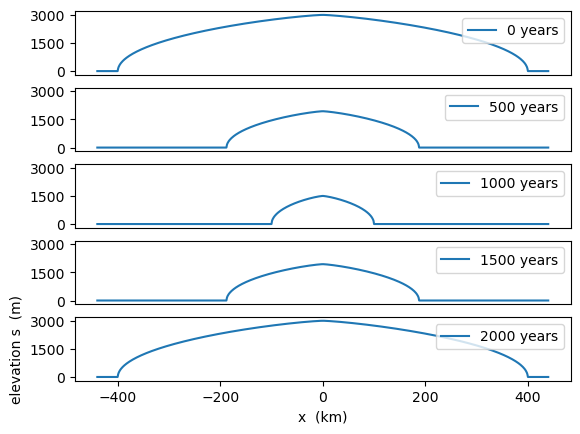
\includegraphics[width=0.75\textwidth]{surfacesnaps}
\caption{Surface elevation at five times in $0\le t \le 2000$ a.}
\label{surfacesnaps}
\end{figure}

The next step in constructing exact formulas for surface kinematics requires a choice about ice dynamics.  A formula for the surface value of velocity must come from assumptions about ice flow, and we will use the velocity generated from the shallow ice approximation (SIA), which went into the construction of the Bueler profile \cite[section 5.3]{vanderVeen2013}.  On the other hand, once we switch to thinking about inversion for CMB we will be assuming that the surface velocity is observed and its physical source does not really matter.

The central SIA formula gives the horizontal ice velocity as a function of the ice thickness, the surface elevation, and the $z$ coordinate \cite{GreveBlatter2009,vanderVeen2013}; see also equation (24) in my notes.  Here $s=H$ and $n=3$ is an odd integer so we may write:
\begin{equation}
u(t,x,z) = - \gamma \left(s(t,x)^{n+1} - (s(t,x)-z)^{n+1}\right) \left(\frac{\partial s}{\partial x}(t,x)\right)^n \label{siaxz}
\end{equation}
where $\gamma = 2 A (\rho g)^n / (n+1)$.  The value at the surface is simpler; it arises by substituting $z=s(t,x)$:
\begin{equation}
u|_s(t,x) = u(t,x,s(t,x)) = - \gamma s(t,x)^{n+1} \left(\frac{\partial s}{\partial x}(t,x)\right)^n \label{siasurfacex}
\end{equation}
Using formulas \eqref{sformula} and \eqref{dsdxformula} completes the computation of the surface value of the horizontal velocity.

Next we need $w|_s$, the surface value of the vertical velocity.  FIXME

\small
\bigskip
\bibliography{syntheticglacier}
\bibliographystyle{siam}
\end{document}
